\documentclass[12pt]{article}
\usepackage[utf8]{inputenc}
\usepackage[usenames]{color}
\usepackage[margin=1in]{geometry} 
\usepackage{amsmath,amsthm,amssymb,graphicx,mathtools,tikz,hyperref, pgfplots, listings, pdfpages}
\usetikzlibrary{positioning}
\newcommand{\n}{\mathbb{N}}
\newcommand{\z}{\mathbb{Z}}
\newcommand{\q}{\mathbb{Q}}
\newcommand{\cx}{\mathbb{C}}
\newcommand{\real}{\mathbb{R}}
\newcommand{\field}{\mathbb{F}}
\newcommand{\ita}[1]{\textit{#1}}
\newcommand{\com}[2]{#1\backslash#2}
\newcommand{\oneton}{\{1,2,3,...,n\}}
\newcommand\idea[1]{\begin{gather*}#1\end{gather*}}
\newcommand\ef{\ita{f} }
\newcommand\eff{\ita{f}}
\newcommand\proofs[1]{\begin{proof}#1\end{proof}}
\newcommand\inv[1]{#1^{-1}}
\newcommand\setb[1]{\{#1\}}
\newcommand\en{\ita{n }}
\newcommand{\vbrack}[1]{\langle #1\rangle}


\newenvironment{theorem}[2][Teorema]{\begin{trivlist}
\item[\hskip \labelsep {\bfseries #1}\hskip \labelsep {\bfseries #2.}]}{\end{trivlist}}
\newenvironment{lemma}[2][Lema]{\begin{trivlist}
\item[\hskip \labelsep {\bfseries #1}\hskip \labelsep {\bfseries #2.}]}{\end{trivlist}}
\newenvironment{exercise}[2][Ejercicio]{\begin{trivlist}
\item[\hskip \labelsep {\bfseries #1}\hskip \labelsep {\bfseries #2.}]}{\end{trivlist}}
\newenvironment{reflection}[2][Reflexión]{\begin{trivlist}
\item[\hskip \labelsep {\bfseries #1}\hskip \labelsep {\bfseries #2.}]}{\end{trivlist}}
\newenvironment{proposition}[2][Proposición]{\begin{trivlist}
\item[\hskip \labelsep {\bfseries #1}\hskip \labelsep {\bfseries #2.}]}{\end{trivlist}}
\newenvironment{corollary}[2][Corolario]{\begin{trivlist}
\item[\hskip \labelsep {\bfseries #1}\hskip \labelsep {\bfseries #2.}]}{\end{trivlist}}
 \hypersetup{
 colorlinks,
 linkcolor=blue
 }

\renewcommand{\ttdefault}{pcr}
\lstdefinestyle{C}{language=C,
    basicstyle=\ttfamily,
    keywordstyle=\bfseries,
    showstringspaces=false,
    morekeywords={include, printf},
	keepspaces=true,numbers=left,xleftmargin=2em,frame=shadowbox,framexleftmargin=0 em, rulesepcolor = \color{black}
}
\lstdefinestyle{linuxterminal}{language=bash,
    basicstyle=\ttfamily,
    keywordstyle=\bfseries,
    showstringspaces=false,
    morekeywords={include, printf},
	keepspaces=true,
	frame=TLRB
}


\begin{document}
	\date{16-04-2018}
	
	
	\title{\textbf{\textcolor{red}{INFORME PRÁCTICA 3}}}
	\author{Alejandro Santorum Varela - alejandro.santorum@estudiante.uam.es\\David Cabornero Pascual - david.cabornero@estudiante.uam.es\\Sistemas Operativos - Pareja 7\\Universidad Autónoma de Madrid}
	\maketitle
	
	\tableofcontents
	
	\newpage
	
\section{Introducción}
Ese documento recoge los ejercicios realizados en la tercera práctica de Sistemas Operativos.\\\\
Para cada ejercicio se comentará su diseño, su funcionalidad detalla y/o un análisis de las diferentes decisiones tomadas a la hora de enfrentarse a los problemas o dificultades encontradas.\\

\section{Ejercicio 2}
El primer ejercicio se basa en el concepto de \textbf{condición de carrera}: el resultado final de un ejercicio con múltiples procesos ejecutándose depende de la secuencia de acción de dichos procesos, provocando que el resultado pueda variar si las varibales compartidas no están bien protegidas.\\

Se nos pide realizar un ejercicio que cree tantos procesos como indique el usuario por línea de comandos. Cada proceso una vez creado dormirá durante un tiempo aleatorio, y a continuación solicitará al usuario que dé de alta a un cliente (nombre), incrementará la variable compartida en una unidad y enviará al proceso padre la señal SIG\_USR1 para indicar que el proceso ha acabado.\\

Tal como se plantea este ejercicio podemos sostener que tiene algunas fujas de corrección. Por un lado, el tiempo de creación de los procesos hijos es insignificante, humanamente hablando, por lo que todos los procesos pedirán al usuario dar de alta un cliente a la vez. Por otro lado, no hay nada protegiendo la variable compartida; si no fuera por el hecho que lo único que hacen es incrementarla (podrían decrementarla algunos y incrementarla otros procesos), podríamos tener diferentes resultados.\\

A continuación mostramos una salida que ejemplifica lo dicho anteriormente:
\begin{center}
	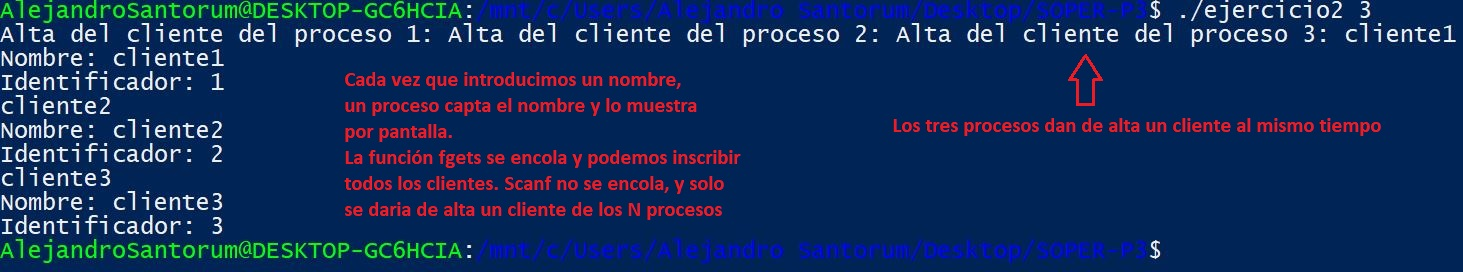
\includegraphics[scale=0.86]{ej2.JPG}
\end{center}
Se comenta en la imagen, pero podemos enfatizarlo: en nuestro programa, aunque todos los procesos nos pidan un nombre, la función fgets(...) se encola y nos permite introducirlos todos tal y como vemos en la imagen. Si utilizásemos la función scanf(...) esto no pasaría y solo podríamos introducir un nombre, y $N-1$ procesos fallarían estrepitosamente

\section{Ejercicio 2 mejorado}
Como continuación del ejercicio 2, tenemos que mejorarlo para que no se produzcan los percances comentados, utilizando lo que sabemos de memoria compartida y semáforos. Esta solución la podemos encontrar en el ejercicio2\_solved.\\

Básicamente lo que hacemos es crear un semáforo. Mientras un proceso pida un cliente, ningún otro proceso podrá hacerlo. Así pues, cuando un proceso llega a la zona crítica baja el semáforo que será levantado cuando el proceso padre haya dado de alta el nuevo cliente.\\

Comentar que iniciarlmente se producían algunos errores con los semáforos (tal y como te comentamos en clase). En un principio era debido a que el sistema no funciona muy bien cuando operamos sobre un semáforo en procesos distintos (por ejemplo, cuando uno lo baja y otro lo sube). No obstante, después de leer varios artículos y posts por internet junto con el man de C, descubrimos, con la colaboración de otras parejas, que la flag \textbf{SEM\_UNDO} no funciona tal y como se muestra en la documentación y que cuando un proceso hijo finaliza envía una señal al padre, \texttt{System call}, produce ciertos fallos en los semáforos. \\

Comentar que este percance ya se había tenido en la práctica anterior con el ejercicio 9, y que había sido solucionado con una espera activa y la bandera \textbf{IPC\_NOWAIT}. En esta hemos mejorado y podemos controlar más robustamente los errores ya que no usamos espera activa, y usamos en el campo flag \textbf{0}.\\

Ahora mostramos la salida del programa mejorado:
\begin{center}
	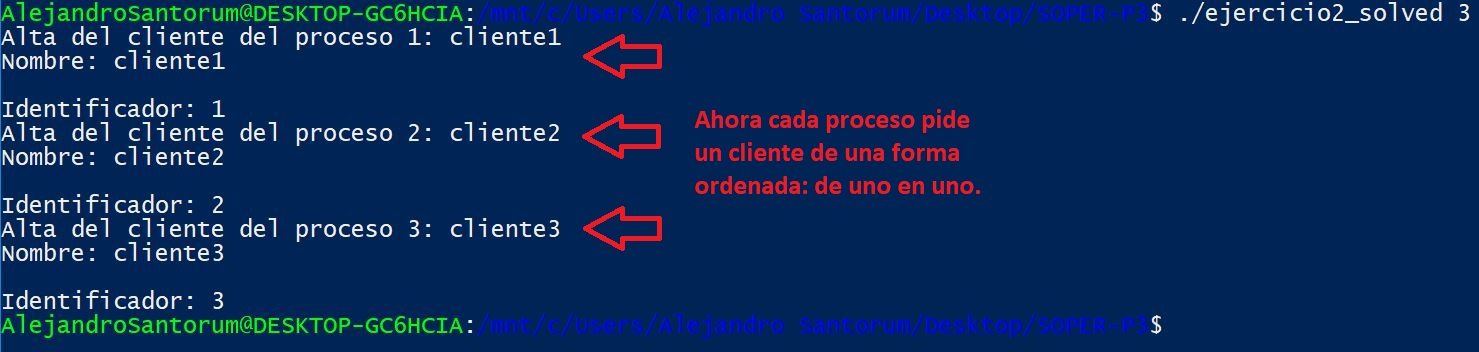
\includegraphics[scale=0.86]{ej2_solved.JPG}
\end{center}


\section{Ejercicio 3}
El ejercicio 3 es el problema del productor-consumidor. En este caso solo necesitamos dos procesos: un productor que introducirá caracteres y los introducirá en un array, y un consumidor, que retirará los caracteres y los mostrará por pantalla.\\

Necesitamos tres semáforos: uno para indicar cuando el array (que simula una estantería de productos) está lleno, otro para indicar cuando el array o estantería está vacío, y por último un semáforo mutex para proteger las variables conflictivas (sección crítica) y para permitir que un único proceso tenga acceso al array en un instante determiando.\\

· \textbf{PRODUCTOR}: down(vacio) $>$ down(mutex) $>$ \texttt{sección crítica}-producir\_producto() $>$ up(mutex) $>$ up(lleno)\\

· \textbf{CONSUMIDOR}: down(lleno) $>$ down(mutex) $>$ \texttt{sección crítica}-consumir\_producto() $>$ up(mutex) $>$ up(vacio)\\

Comentar que la implementación de este ejercicio se ha generalizado: el usuario debe introducir el tamaño del array por parámetro de entrada del programa. El resultado va a ser el mimso, pero un tamaño menor hará que los semáforos que controlan el tamaño del array trabajen más durantemente para que un productor no produzca si la estantería está llena o un consumidor no consuma si no hay productos.\\ Por otro lado, los productos son producidos circularmente, empezamos con la A hasta la Z y después continuamos con los números desde el 0 al 9. Una vez completado el ciclo, volvemos a empezar por la A. No obstante, para ceñirse al enunciado hemos puesto una constante (define) a 36, que es el número de productos a producir y posteriormente a consumir. Si quisésemos producir-consumir más que un ciclo, solo tendríamos que cambiar esta constante.\\

Ahora abajo mostramos la salida del programa:
\begin{center}
	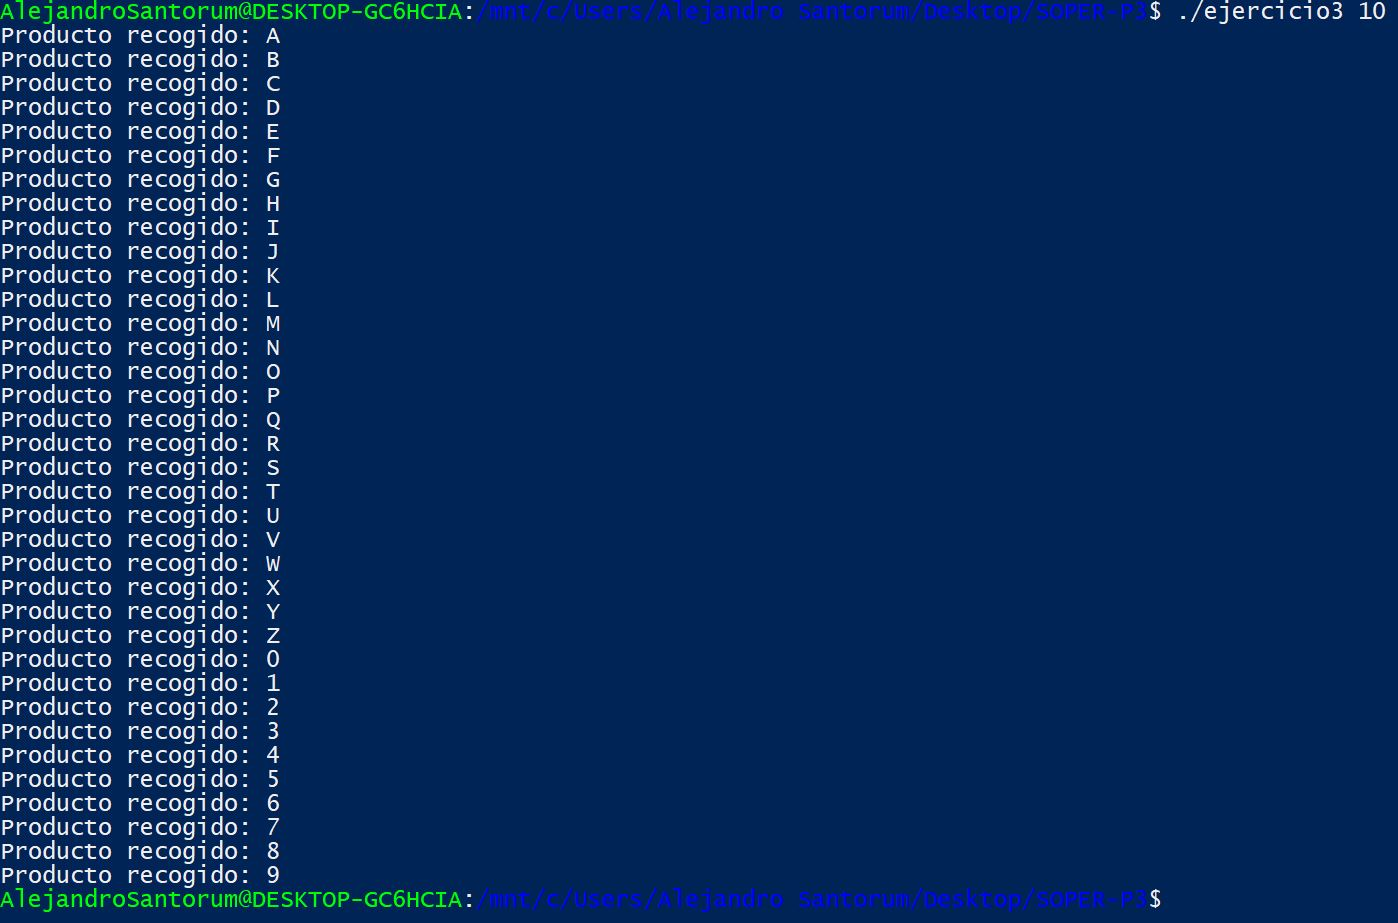
\includegraphics[scale=0.86]{ej3.JPG}
\end{center}


\section{Ejercicio 4}
El ejercicio 4 podríamos considerarlo como una instancia muy sencilla del problema de lectores-escritores. Sin embargo, no podemos decir al 100\% que sea así, ya que el lector y el escritor no trabajan a la vez (tal y como indica el enunciado), por lo que no tenemos que utilizar semáforos ni tener cuidado con la concurrencia.\\

El obetivo principal de este ejercicio es iniciarse con la función mmap(...) de C.\\

Se nos pide iniciar un hilo que escriba en un fichero un número aleatorio entre 1000 y 2000 de números aleatorios entre 100 y 1000. Una vez que haya acabado, el proceso principal iniciará otro hilo, el cual utilizará mmap(...) para leer el contenido del fichero.\\

Comentar que este ejercicio se podría haber hecho de varias formas: en escritor también podría haber escrito ayudándose de la función mmap(...). Nosotros no lo hemos hecho así. Por otro lado, nosotros hemos abierto el fichero en el proceso padre y al segundo hilo le hemos pasado el descriptor del fichero por parámetro, pero se podría haber pasado el nombre del fichero y en el hilo obtener el descriptor del fichero con open(...).\\

Independientemente de lo anterior, el resultado final es idéntico, y aquí mostramos la salida:
\begin{center}
	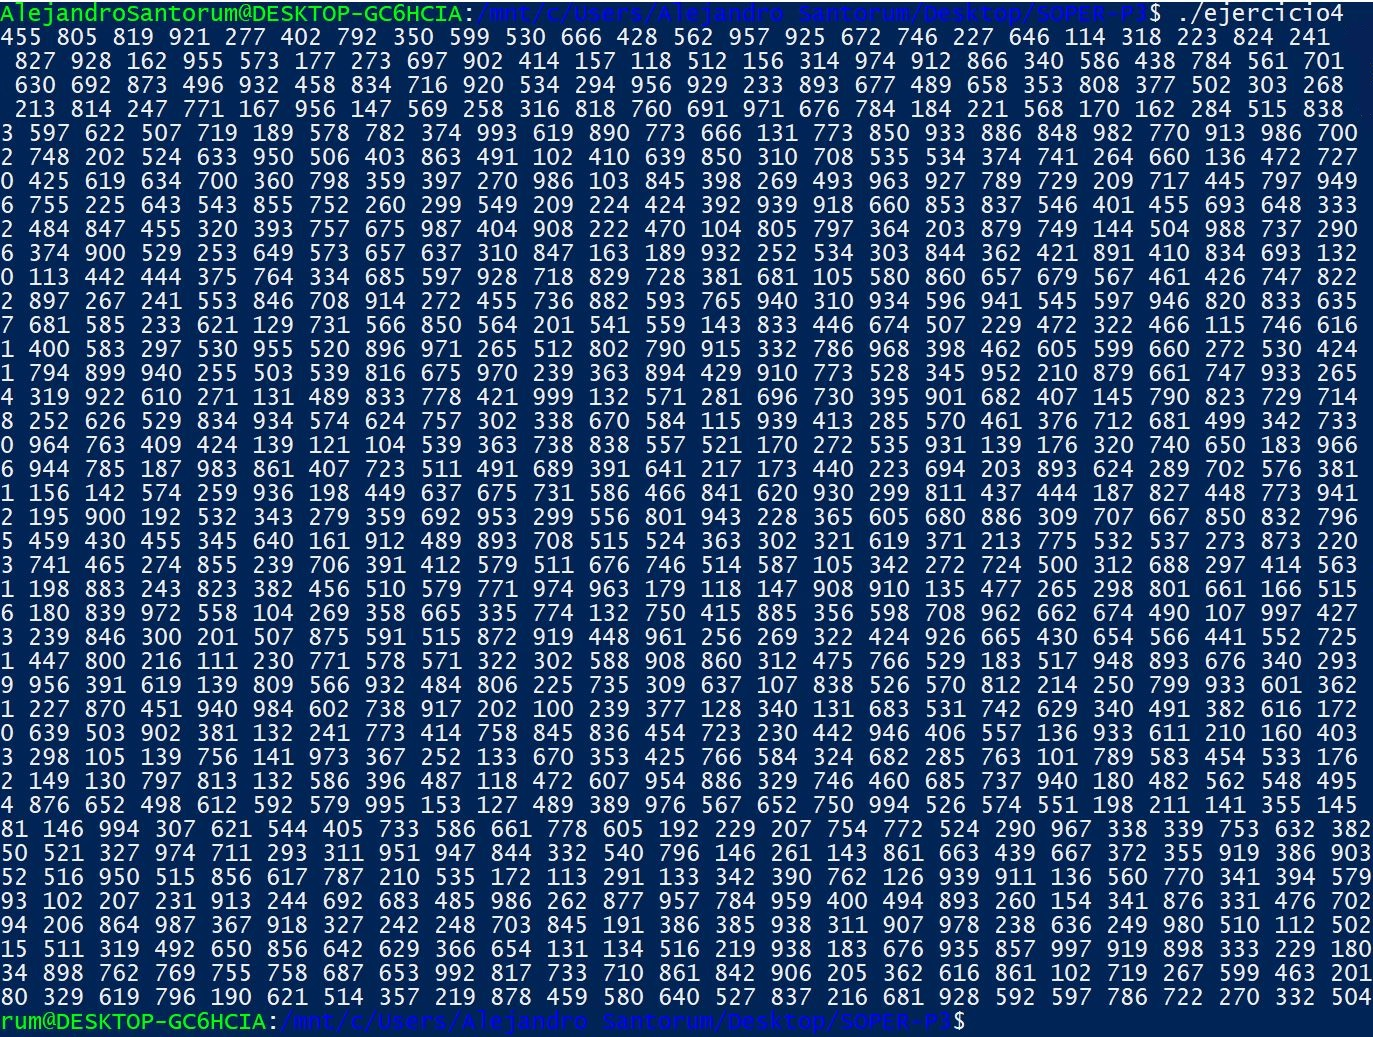
\includegraphics[scale=0.85]{ej4.JPG}
\end{center}


\section{Ejercicio 5}
Finalmente llegamos al ejercicio final de la práctica. Este se basa en el aprendizaje de las funciones de las colas de mensajes.\\

El objetivo del ejercicio es: un proceso A lee de un fichero de entrada texto e introduce en la cola de mensajes trozos del texto de longitud máxima de 2KB. El proceso B coge de la cola de mensajes los trozos de texto, los transforma escribiendo la siguiente letra de cada caracter y se lo envía al proceso C a través de la cola de mensajes. Finalmente, el proceso C lee de la cola de mensajes el texto modificado por B y lo escribe en un fichero de salida.\\

Comentar en primer lugar que para que el proceso B sepa que ya ha finalizado de computar todos los trozos de texto el proceso A le envía una señal cuando A haya acabado. Sin embargo, A puede haber acabado pero B no, por lo que B tiene que comprobar que, además de que A haya acabado, la cola de mensajes este vacía. Esto ocurre simétricamente para el proceso C y el proceso B.\\

Para conocer el número de mensajes restantes en la cola se ha utilizado msgctl con la flag textbf{IPC\_STAT} que nos devuelve información de la cola de mensajes. Debido a que el número obtenido de mensajes en la cola con esta función es la suma de todos los mensajes de diferente tipo, hemos tenido que crear dos colas independientes: una para pasar mensajes de A a B y otra para B y C. Esto es para poder saber cuando finalizar los procesos B y C.\\

Aunque utilicemos dos colas independientes, los mensajes entre A y B son del tipo 1, y los mensajes entre B y C son de tipo 2. Esto es así para demostrar que sabemos usar mensajes de diferente tipo, aunque para este ejercicio con esta implementación no sea necesario.\\

Este ejercicio \texttt{no produce ninguna salida por terminal}, pero adjuntamos dos ficheros de texto, "origen.txt" y "destino.txt", que ya han sido utilizados por el programa, por lo que tienen la salida esperada, la cual se puede comprobar que es del mismo tamaño y que cada letra del origen.txt es la anterior a la del destino.txt.\\

\textbf{NOTA}: En la entrega anticipada se detectó un warning que no había saltado en nuestros ordenadores, a pesar de usar la flag -Wall. Después de buscar información exhaustivamente, descubrimos que esto se debe a un \emph{bug} de aparición reciente. A continuación mostramos los reportes de \emph{StackOverflow} y de una página especializada en \emph{bugs}:
\begin{center}
	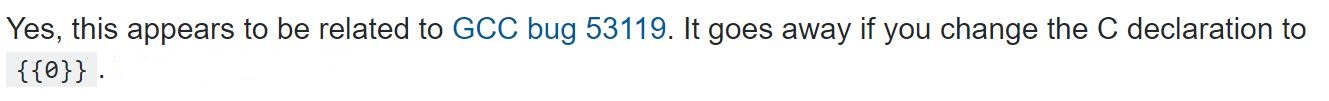
\includegraphics[scale=0.9]{sofSolution.JPG}
\end{center}
\begin{center}
	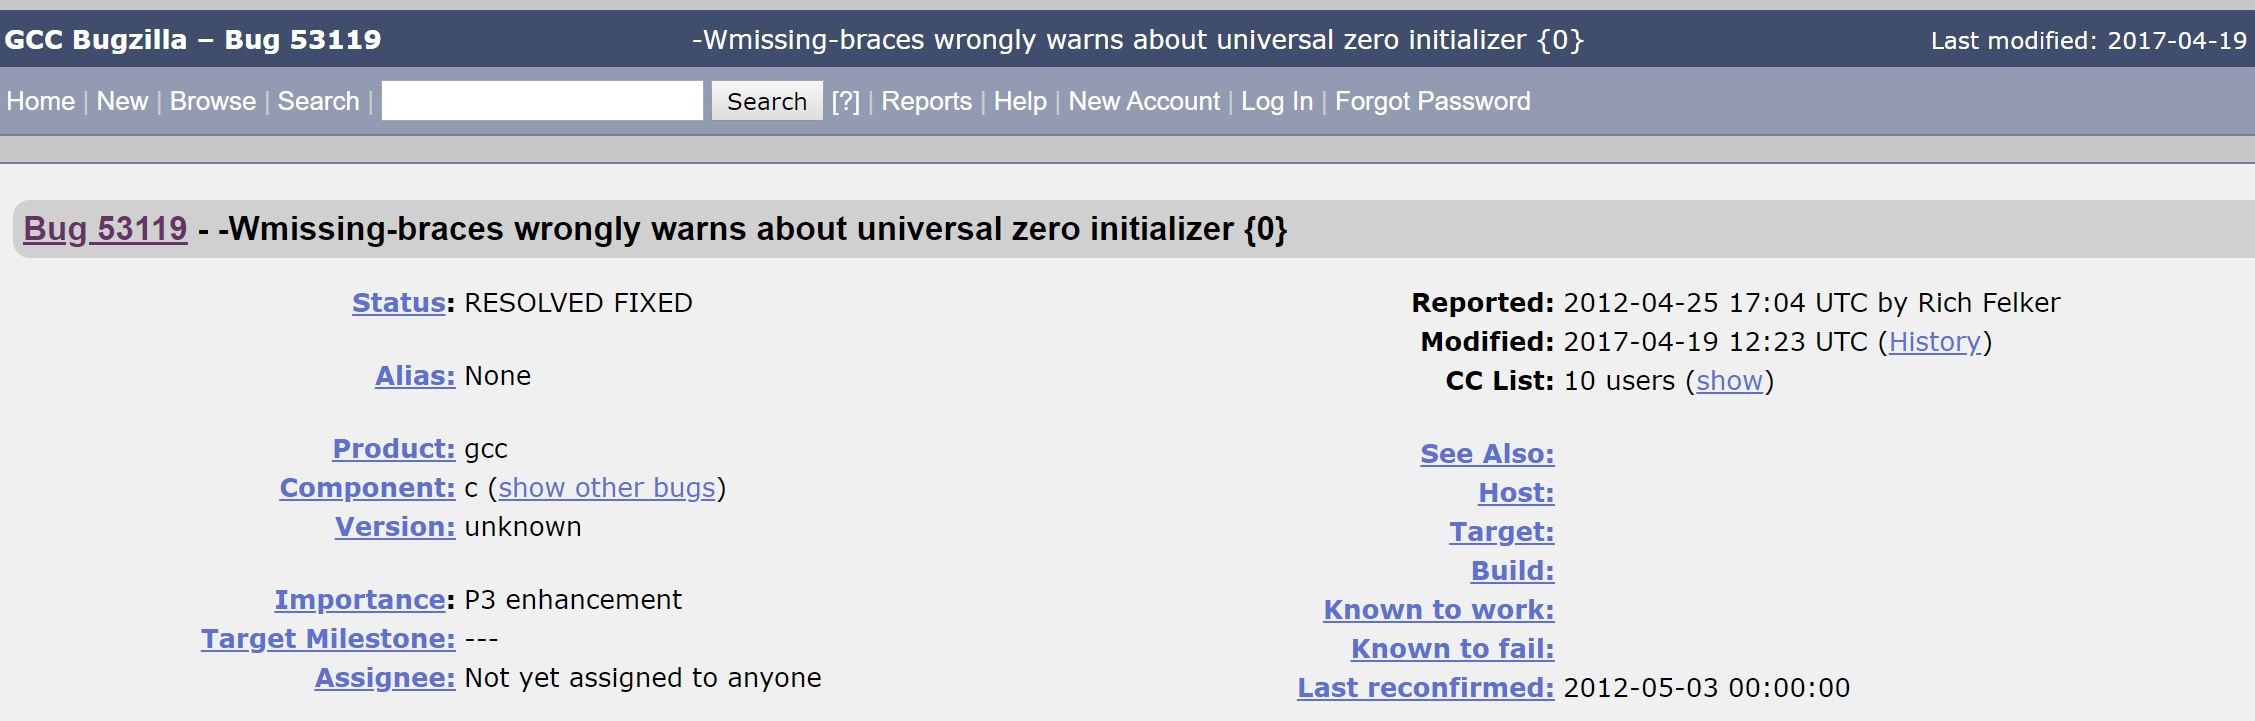
\includegraphics[scale=0.55]{bug.JPG}
\end{center}
Utilizando lo anterior hemos modificado nuestro código a esto. La compilación a nosotros nos sigue resultando perfecta, pero no hemos podido comprobar al $100\%$ que se soluciona el problema. Aún así, \emph{StackOverflow} suele proporcionar muy buenas soluciones, y no fueron pocos los usuarios que aconsejaron la mostrada solución.
\begin{center}
	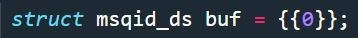
\includegraphics[scale=1]{miSolucion.JPG}
\end{center}


\section{Conclusión}
Esta ha sido una práctica corta pero bastante productiva. Hemos obtenido muy buenas herramientas para el proyecto final y hemos aprendido nuevas formas de comunicar procesos.\\

Posiblemente esta práctica este menos refinada que las dos anteriores debido al poco tiempo que hemos tenido, pero creemos que ha salido todo exitosamente y hemos hecho una buena práctica.\\

Agradecer el trabajo del profesor, que a pesar de tener el tiempo muy limitado, le ha echado un ojo a la entrega de la práctica anticipada.

	
\end{document}